\chapter{Human-guided iterative training \protect\\ of dynamic motions}
In this section, we propose iterative training frameworks for
dynamic motor skills of virtual characters and real robots.
We already introduced an intuitive and interactive system for
developing dynamic controllers of virtual characters,
inspired by human learning process \cite{fitts:1967:hp}.
Further, we want to extend the system to guide a motor skill 
acquition process of real robots, which is also related to
``Learning from Demonstration'' paradigm in robotics.

\section{Prior Work: Iterative Training Of Dynamic Skills Inspired By Human Coaching Techniques}

In our prior work \cite{Ha:2014:ITD},
we introduce an intuitive and interactive framework for developing 
dynamic controllers inspired by how humans learn dynamic motor
skills through progressive process of coaching and practices. 
The user only needs to provide a primitive initial controller and
high-level, human-readable instructions as if
she is coaching a human trainee, while the character has the ability
to interpret the abstract instructions, accumulate the knowledge from
the coach, and improve its skill iteratively. We introduce ``control
rigs'' as an intermediate layer of control module to facilitate the
mapping between high-level instructions and low-level control
variables. Control rigs also utilize the human coach's knowledge to
reduce the search space for control optimization. In addition, we
develop a new sampling-based optimization method, Covariance Matrix
Adaptation with Classification (CMA-C), to efficiently compute control
rig parameters. Based on the observation of human ability to ``learn
from failure'', CMA-C utilizes the failed simulation trials to
approximate an infeasible region in the space of control rig
parameters, resulting a faster convergence for the CMA
optimization. 
Without using motion trajectories, or tuning any parameters,
We demonstrate the design process of complex dynamic
controllers using our framework, including precision jumps, turnaround
jumps, monkey vaults, drop-and-rolls, and wall-backflips 
(\figref{training1_teaser}).


\begin{figure}[htbp]
\center
  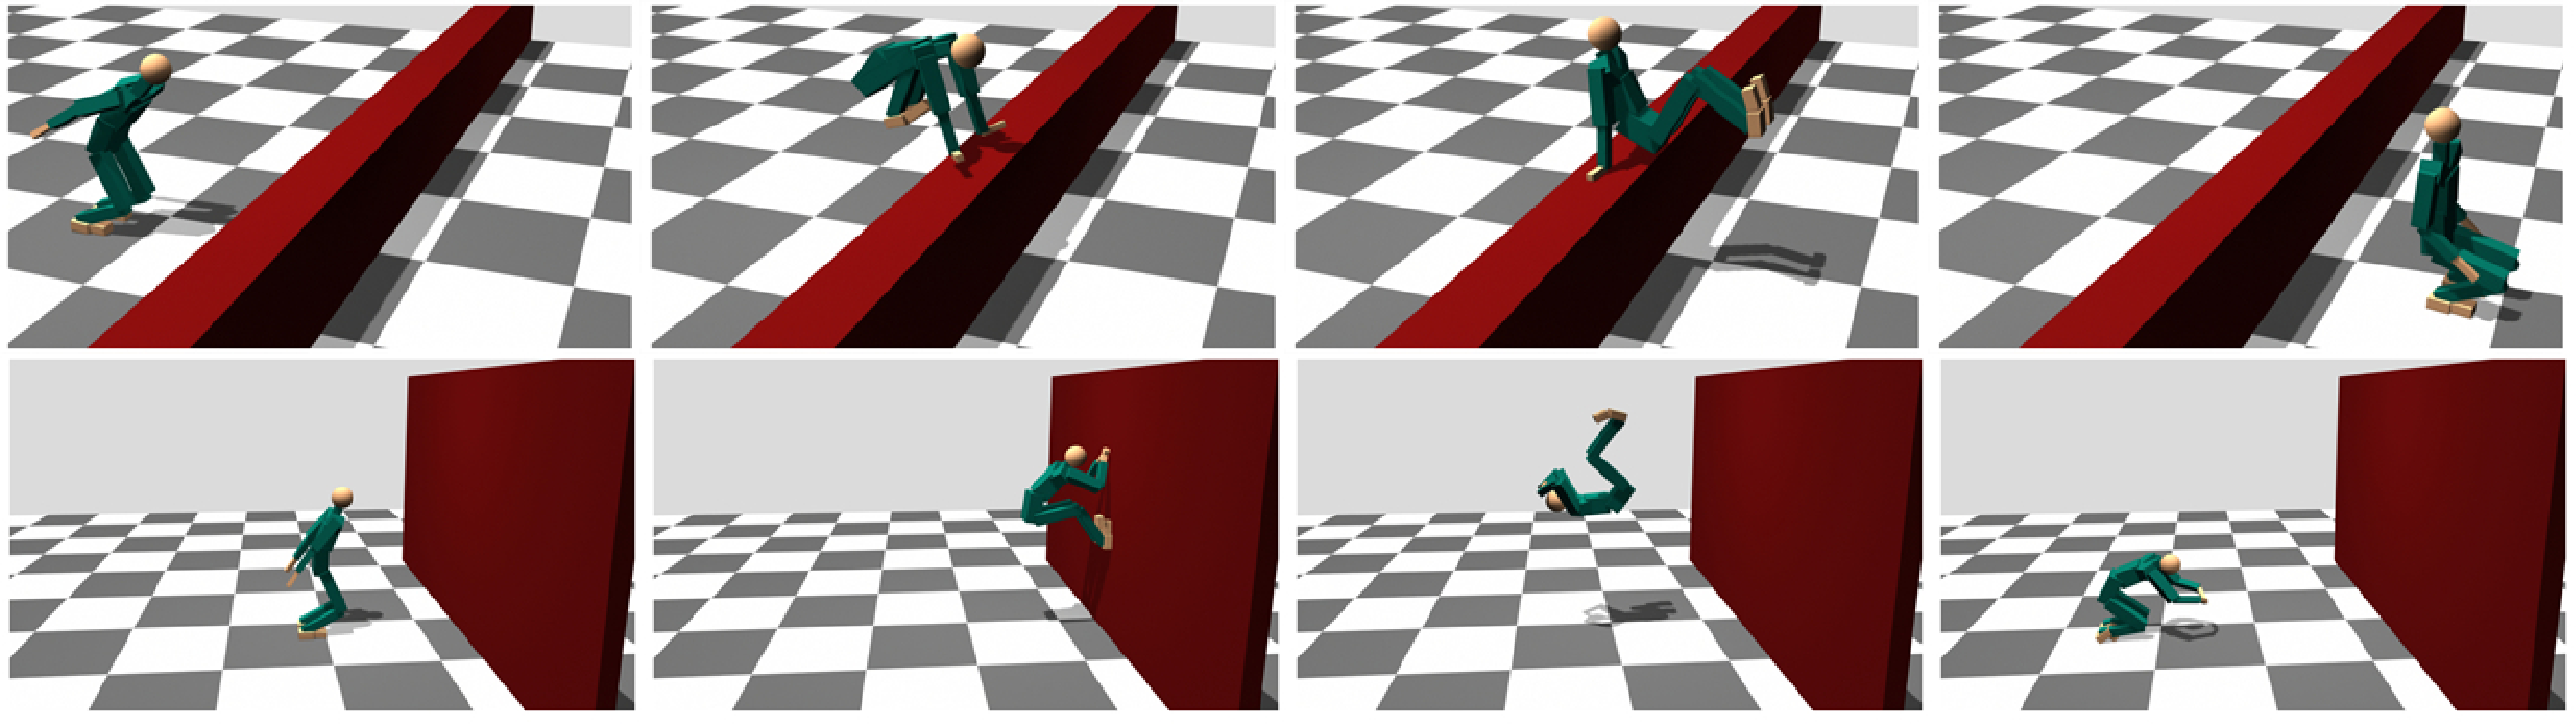
\includegraphics[width=\linewidth]{images/training1_teaser}
  \caption{Monkey vault (Top) and wall-backflip (Bottom).}
 \label{fig:training1_teaser}
\end{figure}


\section{Learning Dynamic Skills in Control Domain for a Humanoid Robot}

\subsection{Problem Description}

In this section, we propose to develop a framework for learning
dynamic motor skills of humanoid robots from user-provided demonstrations 
and instructions, which are common ways to guide a human-trainee.
Within our framework, a coach demonstrates a set of example motions
that consists of joint or mementum trajectories. 
Since trajectories cannot be directly applied to the robots,
instructions are used to interprete the motion to a proper
control space, such a low-dimensional torque space or a control rig 
space \cite{Ha:2014:ITD} that suggested in our previous work.
Finally, we derive a robust control policy from the interpreted
demonstration set by learning an approximation of the state-action mapping.
As a result, we can demonstrate a full-body dynamic motor skills
of humanoid robots under the guidance of human coach.

\subsection{Related Work}

Learning from demonstration (LfD), also known as programming by demonstration,
has been an attractive paradigm for training motor skills to robots.
In this paradigm, a set of examples are provided by human teachers,
and an optimal policy is generated from such examples.
Since the early work of Kuniyoshi \etal \cite{kuniyoshi:1989:TBS},
it has been proven to be effective for training motor skills in
numerous task domains, including object manipulation 
\cite{Atkeson:1997:RLD,Calinon:2007:LRG,Ueda:2010:MNH},
navigation \cite{Konidaris:2011:RLD}, 
full-body motion generation \cite{Kulic:2011:ILF}, and so on.
To increase the robustness, the learned motor skills are further 
generalized using machine learning techniques,
such as gausian mixture model \cite{Calinon:2007:LRG} or
motion primitives \cite{Pastor:2009:LGM}.
However, dynamic motor skills of humanoids have
not been fully examined yet, except the only few works on the
locomotion \cite{Nakanishi:2004:LDA}, which is our target domain
in this proposal.

\subsection{Algorithms}

\paragraph{Domain of learning}

Choosing the right domain of learning is a critical problem 
in ``Learning from Demonstration'' paradigm.
In the literature, one of the most common domains is a set of kinematic
trajectories in joint angles or task spaces.
For instance, Akgun \etal \cite{Akgun:2011:KLD} presented a framework
for learning object manipulation tasks, such as scooping, pouring, or 
placement, from the keyframe data using Sequential Pose Distributions (SPD).
However, joint or torque trajectories cannot be directly applied to the
dynamic skills of the robots  due to the different dynamic properties 
of a coach and a trainee, which can make a huge impact on the motion
with just minor deviations.

To overcome this issue, we hypothesize that learning in the control domain
instead of the kinematic domain would allow straight-forward learning and
roboust behaviors.
To this end, we combine the demonstration with user-provided high-level
instructions, which can help us to identify the proper domain of controls.
The control domain can be a projected low-dimensional control space using
Principal Component Analysis (PCA) or a control rig space, as defined
in \cite{Ha:2014:ITD}.
Especially, control rigs can project the high-dimensional control into
lower dimensions by control multipel degrees of freedoms simultaneously,
and can be easily  easily constructed from a sequence of human-readble 
instructions.
For instance, ``MOVE DOWN'' instruction will add a ``Leg-distance'' rig,
which controls the distance between the root and feet using an inverse
kinematics solver.
We hope that high-level instructions can expedite the learning from
demonstration for dynamic motor skills.

\paragraph{Optimization}

To apply to the trainee, a robot, the control parameters are required to be
optimized to the new dynamic character to follow the user-provided 
examples and instructions.
To optimize the parameters in the simulation environtment, 
it might be easily solved with a standard sampling-based optimization
techniques, such as CMA.
However, deploying the controller to the real robot with hardwares
may require the additional robustness of the controller
due to the noise on the sensors and servos.
Therefore, we may need to ensure the robustness of the solution,
which can be potentially done by  testing the objective value 
with minor perturbations as suggested in Ha \etal \cite{Ha:2013:PSB}.

\subsection{Expected Results}
